\chapter{Phase III - design}

La phase III est la dernière phase du développement clinique d’un nouveau traitement.\\

Les phases III sont toujours des \textbf{essais comparatifs}:
\begin{itemize}
    \item L’idée est de confronter le nouveau traitement au traitement
standard ou à un placebo
    \item L’idée est que les patients du groupe traitement et du groupe
contrôle ne diffère que par leur traitement (\textbf{causalité}).
\end{itemize}

\section{Choix de l’endpoint}

Le choix de l’endpoint est très important et doit se faire en fonction de l’objectif de l’étude. Il est déterminé en fonction du type de maladie et du type de
patients et doit représenter un bénéfice clinique pour le patient. Ce choix va déterminer le type d’analyse. 

\subsection{Primary endpoint}
\begin{itemize}
    \item Endpoint principal
    \item En général : unique, base pour calcul de la taille d’échantillon
    \item De préférence : "Hard" endpoint
\end{itemize}

\subsection{Secondary endpoints}
\begin{itemize}
    \item Endpoints secondaires
     \item En général : plusieurs, attention à la puissance
\end{itemize}


\section{Choix du groupe contrôle}
Lors d'essais cliniques, on fait une comparaison du traitement avec un autre traitement (= traitement de référence) sur une même période, un groupe similaire de patients, et dans des conditions similaires.\\

\begin{center}
    \textbf{Que peut-on considérer comme bras contrôle ?}
\end{center}
\begin{itemize}
    \item un groupe de patients non-traité ?
 \item un groupe de patients traités avec un placebo
 \item un groupe de patients avec un autre traitement connu ?
 \item un groupe de patients avec un autre traitement expérimental ? (Besoin d'un autre groupe de contrôle quand même)
\end{itemize}

\subsection{Unités témoins ou groupe de références}
ensemble des individus servant de comparaisons et qui ne reçoit pas de traitement (ou un placebo) ou qui reçoit un traitement dont les effets sont connues(« traitement standard »)

\subsection{Placebo}

\textbf{Placebo}: substance ayant le même aspect (forme, odeur, couleur, etc) que le traitement étudié, mais étant totalement inactive.

\subsubsection{Effet placebo}
L’effet placebo est souvent lui-même un effet confondant : une personne recevant un placebo, en pensant recevoir une substance active, peut se sentir mieux – simplement parce qu’on lui a administré quelque chose qu’elle croit actif (effet placebo – du latin « je plais »).

\subsubsection{Étude en aveugle}
Étude en aveugle avec un contrôle placebo : on randomise une partie des unités expérimentales à recevoir le traitement étudié et l’autre partie à recevoir un placebo sans que l’unité expérimentale (ou son entourage) ne sache quel traitement a été attribué à quelle unité expérimentale.\\

Il y a \textbf{trois niveaux d'aveugle : }
\begin{figure}[H]
    \centering
    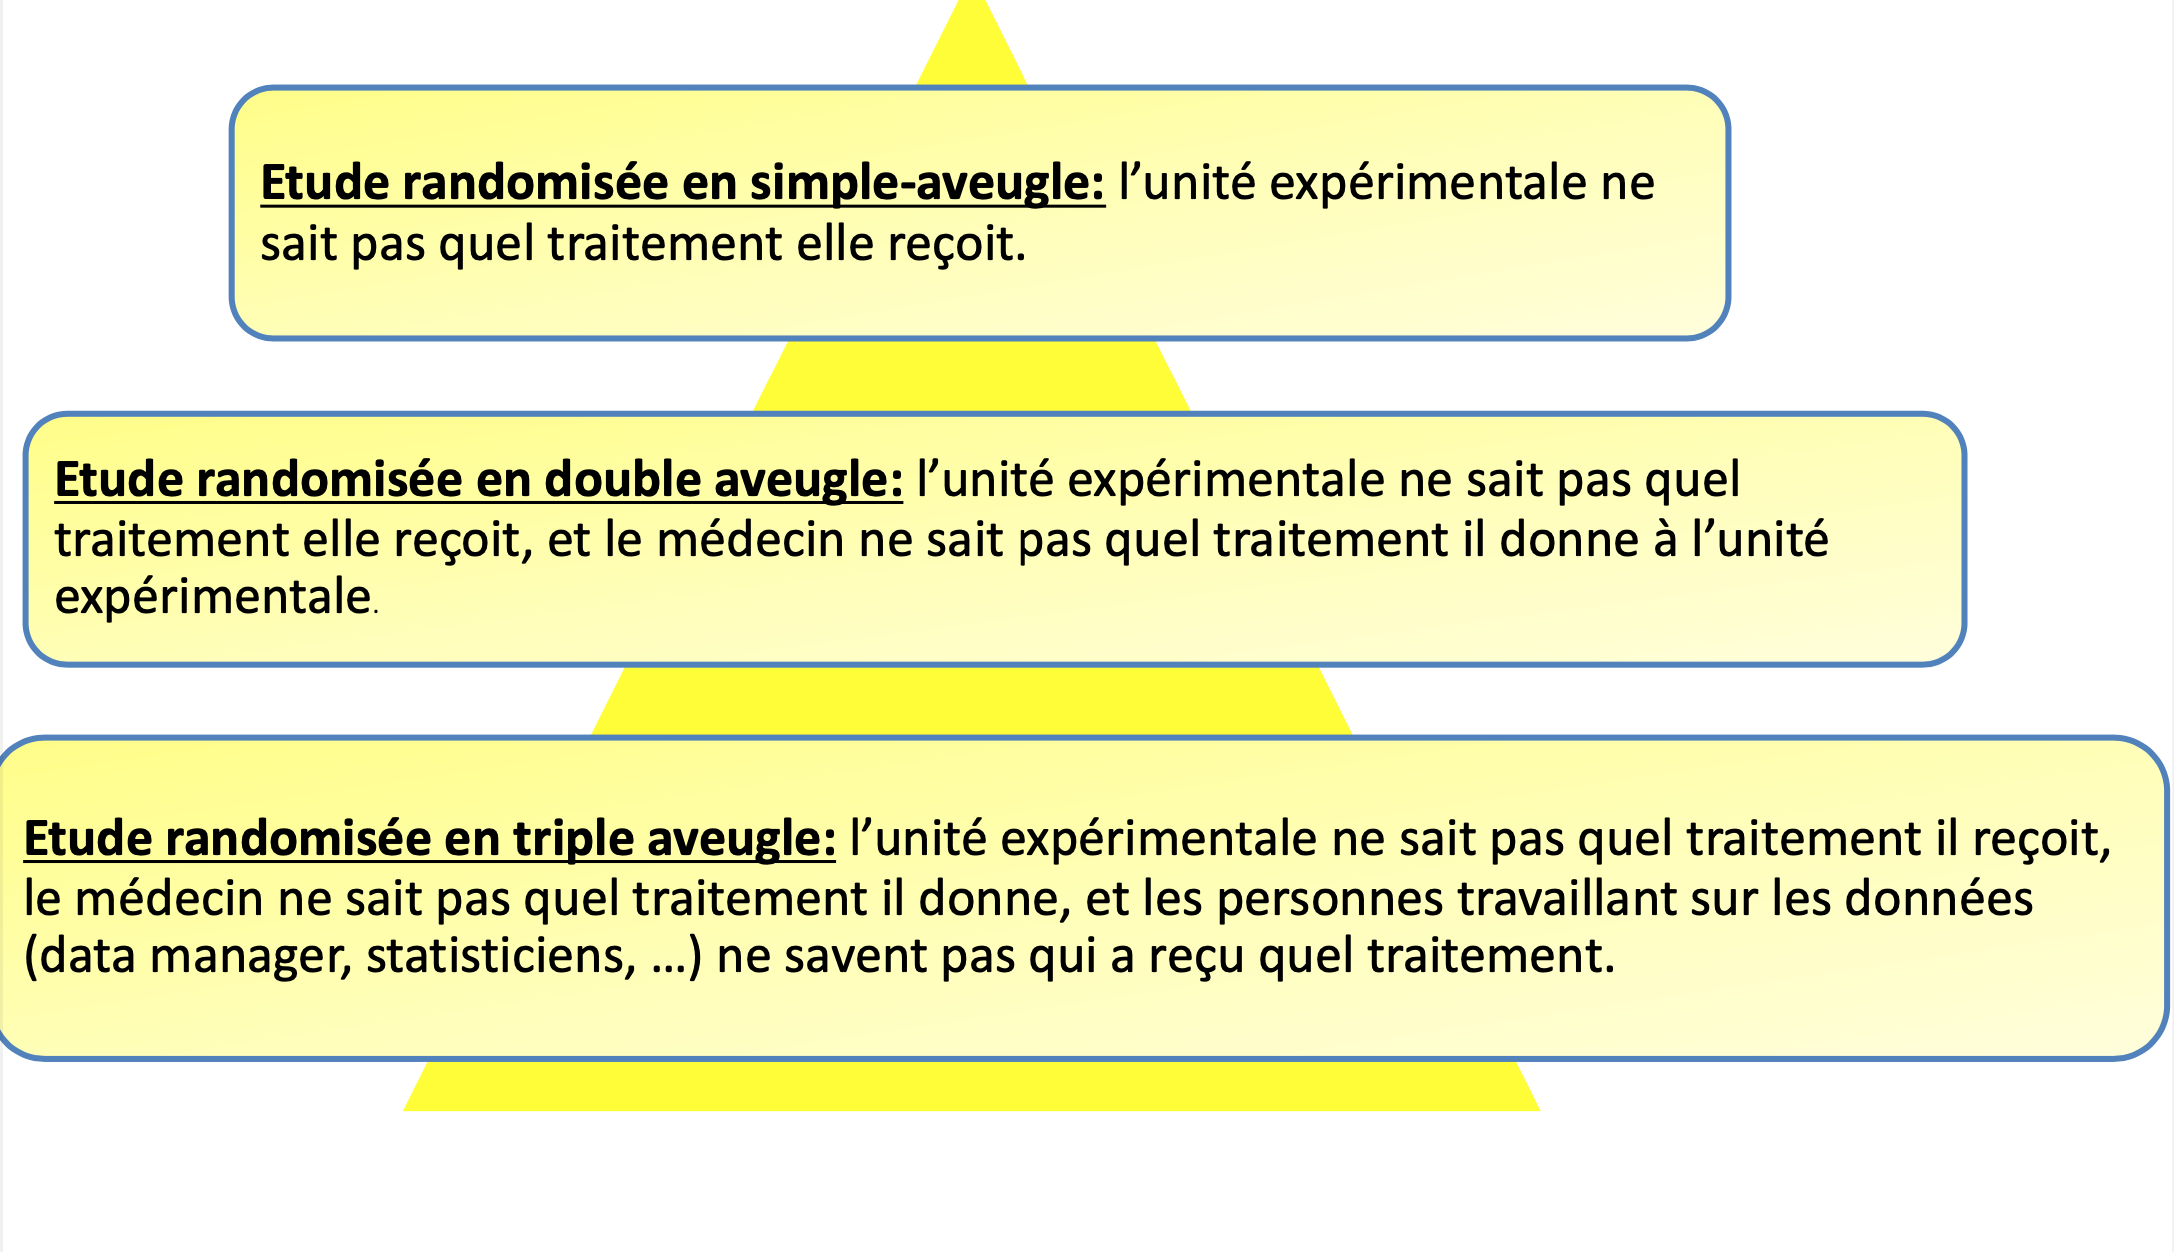
\includegraphics[scale = 0.3]{images/3_blind_levels.png}
    \caption{trois niveaux d'aveugle}
    \label{fig:my_label}
\end{figure}
\begin{enumerate}
    \item  Étude randomisée en simple-aveugle : l’unité expérimentale ne sait pas quel traitement elle reçoit
    \item  Étude randomisée en double aveugle: l’unité expérimentale ne sait pas quel traitement elle reçoit et le médecin ne sait pas quel traitement il donne à l’unité expérimentale.
    \item Étude randomisée en triple aveugle : l’unité expérimentale ne sait pas quel traitement il reçoit, le médecin ne sait pas quel traitement il donne et les personnes travaillant sur les données (data manager, statisticiens, etc) ne savent pas qui a reçu quel traitement.
    
\end{enumerate}
\vspace{0.15cm}



\textbf{\textit{Pourquoi masquer le traitement au patient ?}}\\

Masquer le traitement au patient : balancer l’effet placebo/essais clinique, éviter que le patient ne change de comportement en fonction du treatment, et éviter un découragement du patient si pas randomisé dans le bras souhaité.\\


\textbf{\textit{Pourquoi masquer le traitement à l’équipe médicale ?}}\\


Masquer le traitement à l’équipe médicale  permet de s’assurer que tous les patients seront traités et suivi de la même façon
– Par exemple management des effets secondaires et toxicités, réalisation
d’examens supplémentaires, soutien au patient, collection des
données, évaluation de l’outcome...\\

\textbf{\textit{Pourquoi masquer le traitement à l’équipe responsable de l’essai clinique ?}}\\
Masquer le traitement à l’équipe responsable de l’essai clinique : s’assurer que les décisions prises au cours de l’essai seront prises indépendamment du traitement reçu par le patient, permet d’éviter un suivi de l’effet traitement au cours de l'essai.

Quand on fait un test pas en aveugle. Il peut être difficile, à la fin de l’étude, de conclure si l’effet observé est dû à un réel effet du traitement ou a un effet du placebo. Alors que si l'étude se fait en aveugle. À la fin de l’étude, on peut conclure que  l’effet observé est dû à un effet réel du traitement (puisque l’effet placebo sera le même dans les deux groupes). Par contre, on ne peut pas évaluer l’effet traitement global.\\

\textbf{\textit{Si on est dans une situation ou l’utilisation d’un placebo est éthique, est-ce vraiment toujours possible ?}}\\

Non ce n'est pas toujours possible pour différentes raisons :
\begin{itemize}
    \item Les études avec placebo sont plus compliquée (et plus couteuse) à mettre sur pied
 \item peuvent avoir un recrutement plus difficile (les gens ne veulent pas recevoir de placebo)
 \item ne sont pas toujours possibles :
 \begin{itemize}
     \item soit, car il est impossible de fabriquer un placebo
\item soit parce que l’administration d’un placebo ne serait pas 
éthique
\item soit parce qu’il n’est pas possible de maintenir l’aveugle
 \end{itemize}
 \item ne sont pas toujours utile par exemple si : 
 \begin{itemize}
     \item on considère une maladie pour laquelle l’effet placebo est 
négligeable (cancer, malformation cardiaque, …)
\item l’effet placebo est négligeable sur la mesure utilisée pour 
mesurer l’effet traitement (réduction de la taille de la tumeur, 
survie, …)
\item on peut raisonnablement penser qu’aucun effet placebo n’est 
attendu.
 \end{itemize}
\end{itemize}
\vspace{0.15cm}

Dans certaines situations, il n'est pas éthique de prendre un placebo. Dans le cas où il existe un traitement connu, et qu'il prévient des dommages graves (décès ou morbidités non réversibles).

\begin{figure}[H]
    \centering
    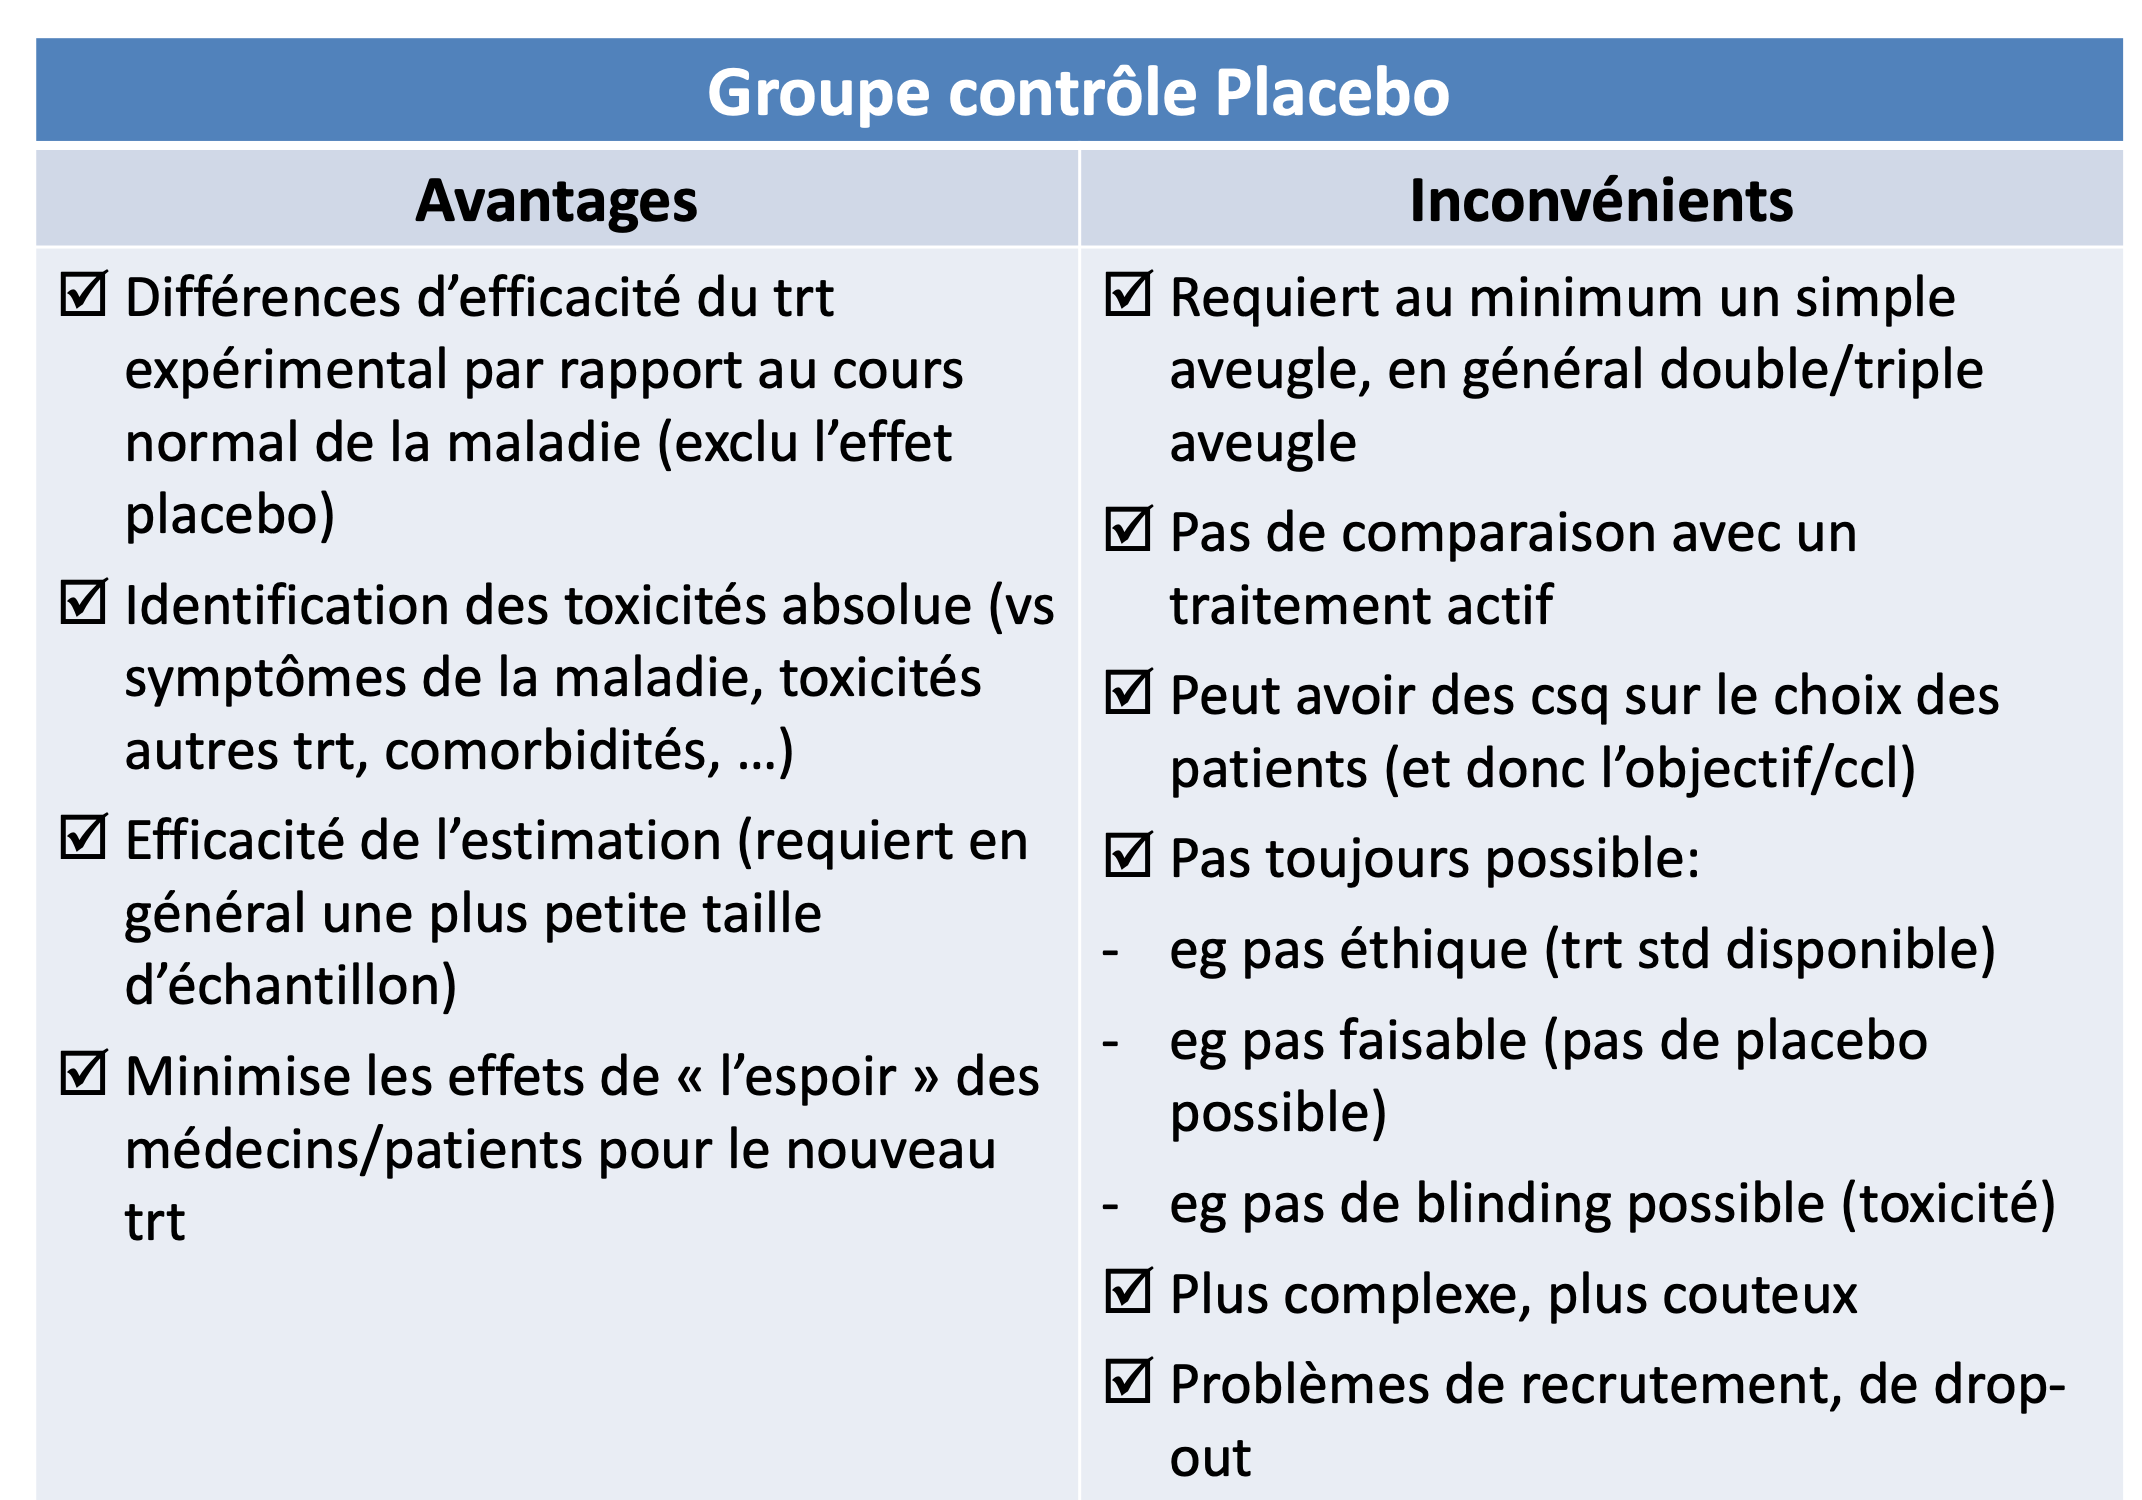
\includegraphics[scale=0.3]{images/placebo.png}
    \caption{}
    \label{fig:my_label}
\end{figure}

\begin{figure}[H]
    \centering
    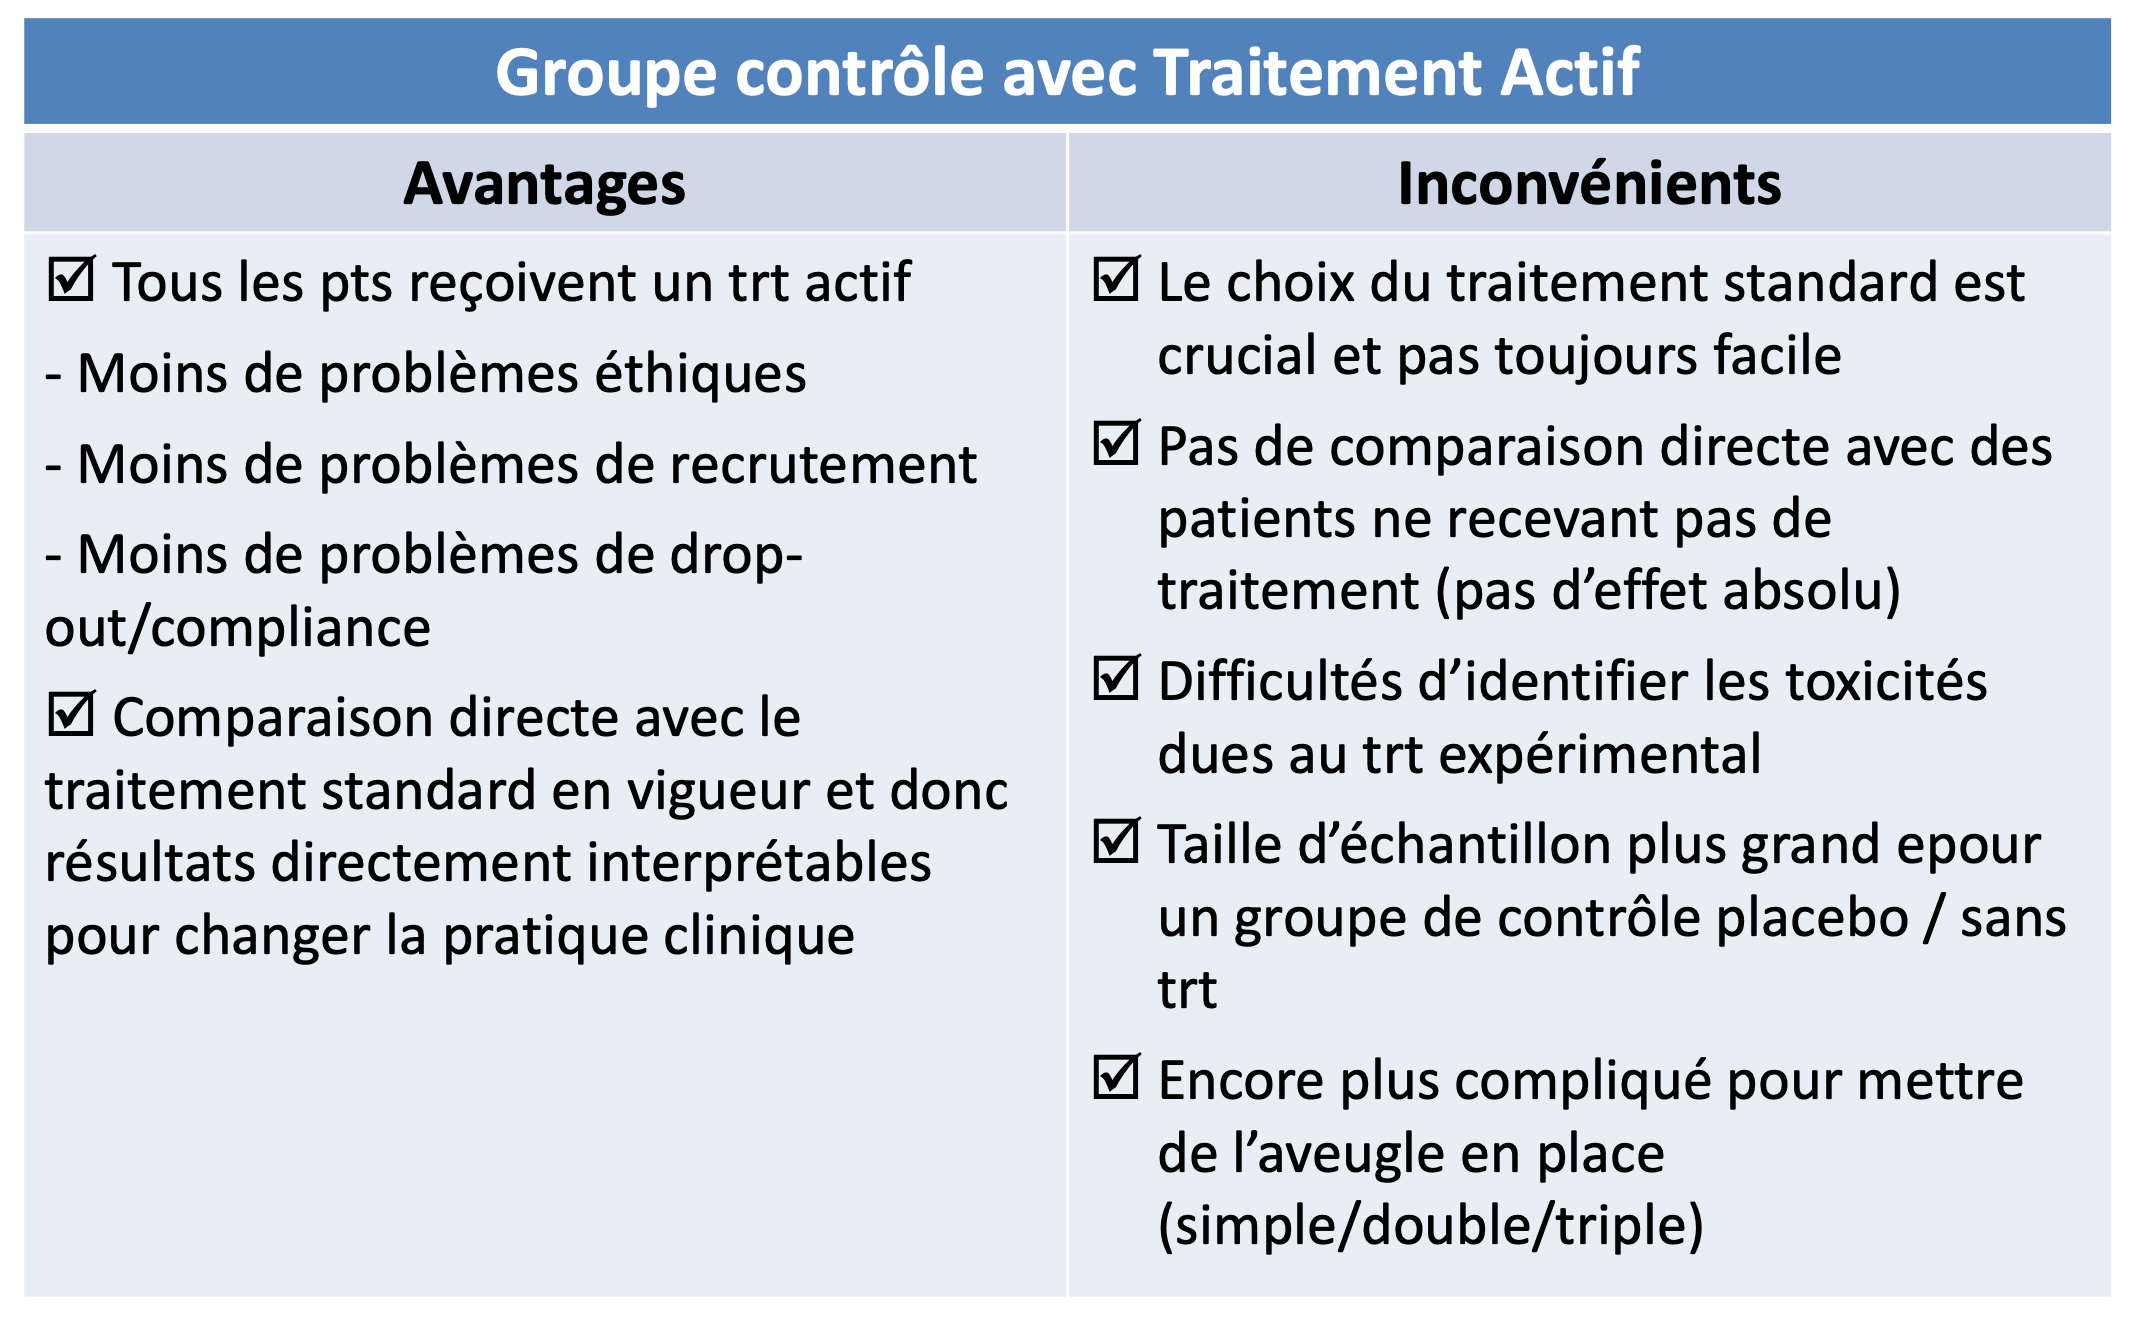
\includegraphics[scale=0.3]{images/actif_treatment.png}
    \caption{}
    \label{fig:my_label}
\end{figure}


\begin{figure}[H]
    \centering
    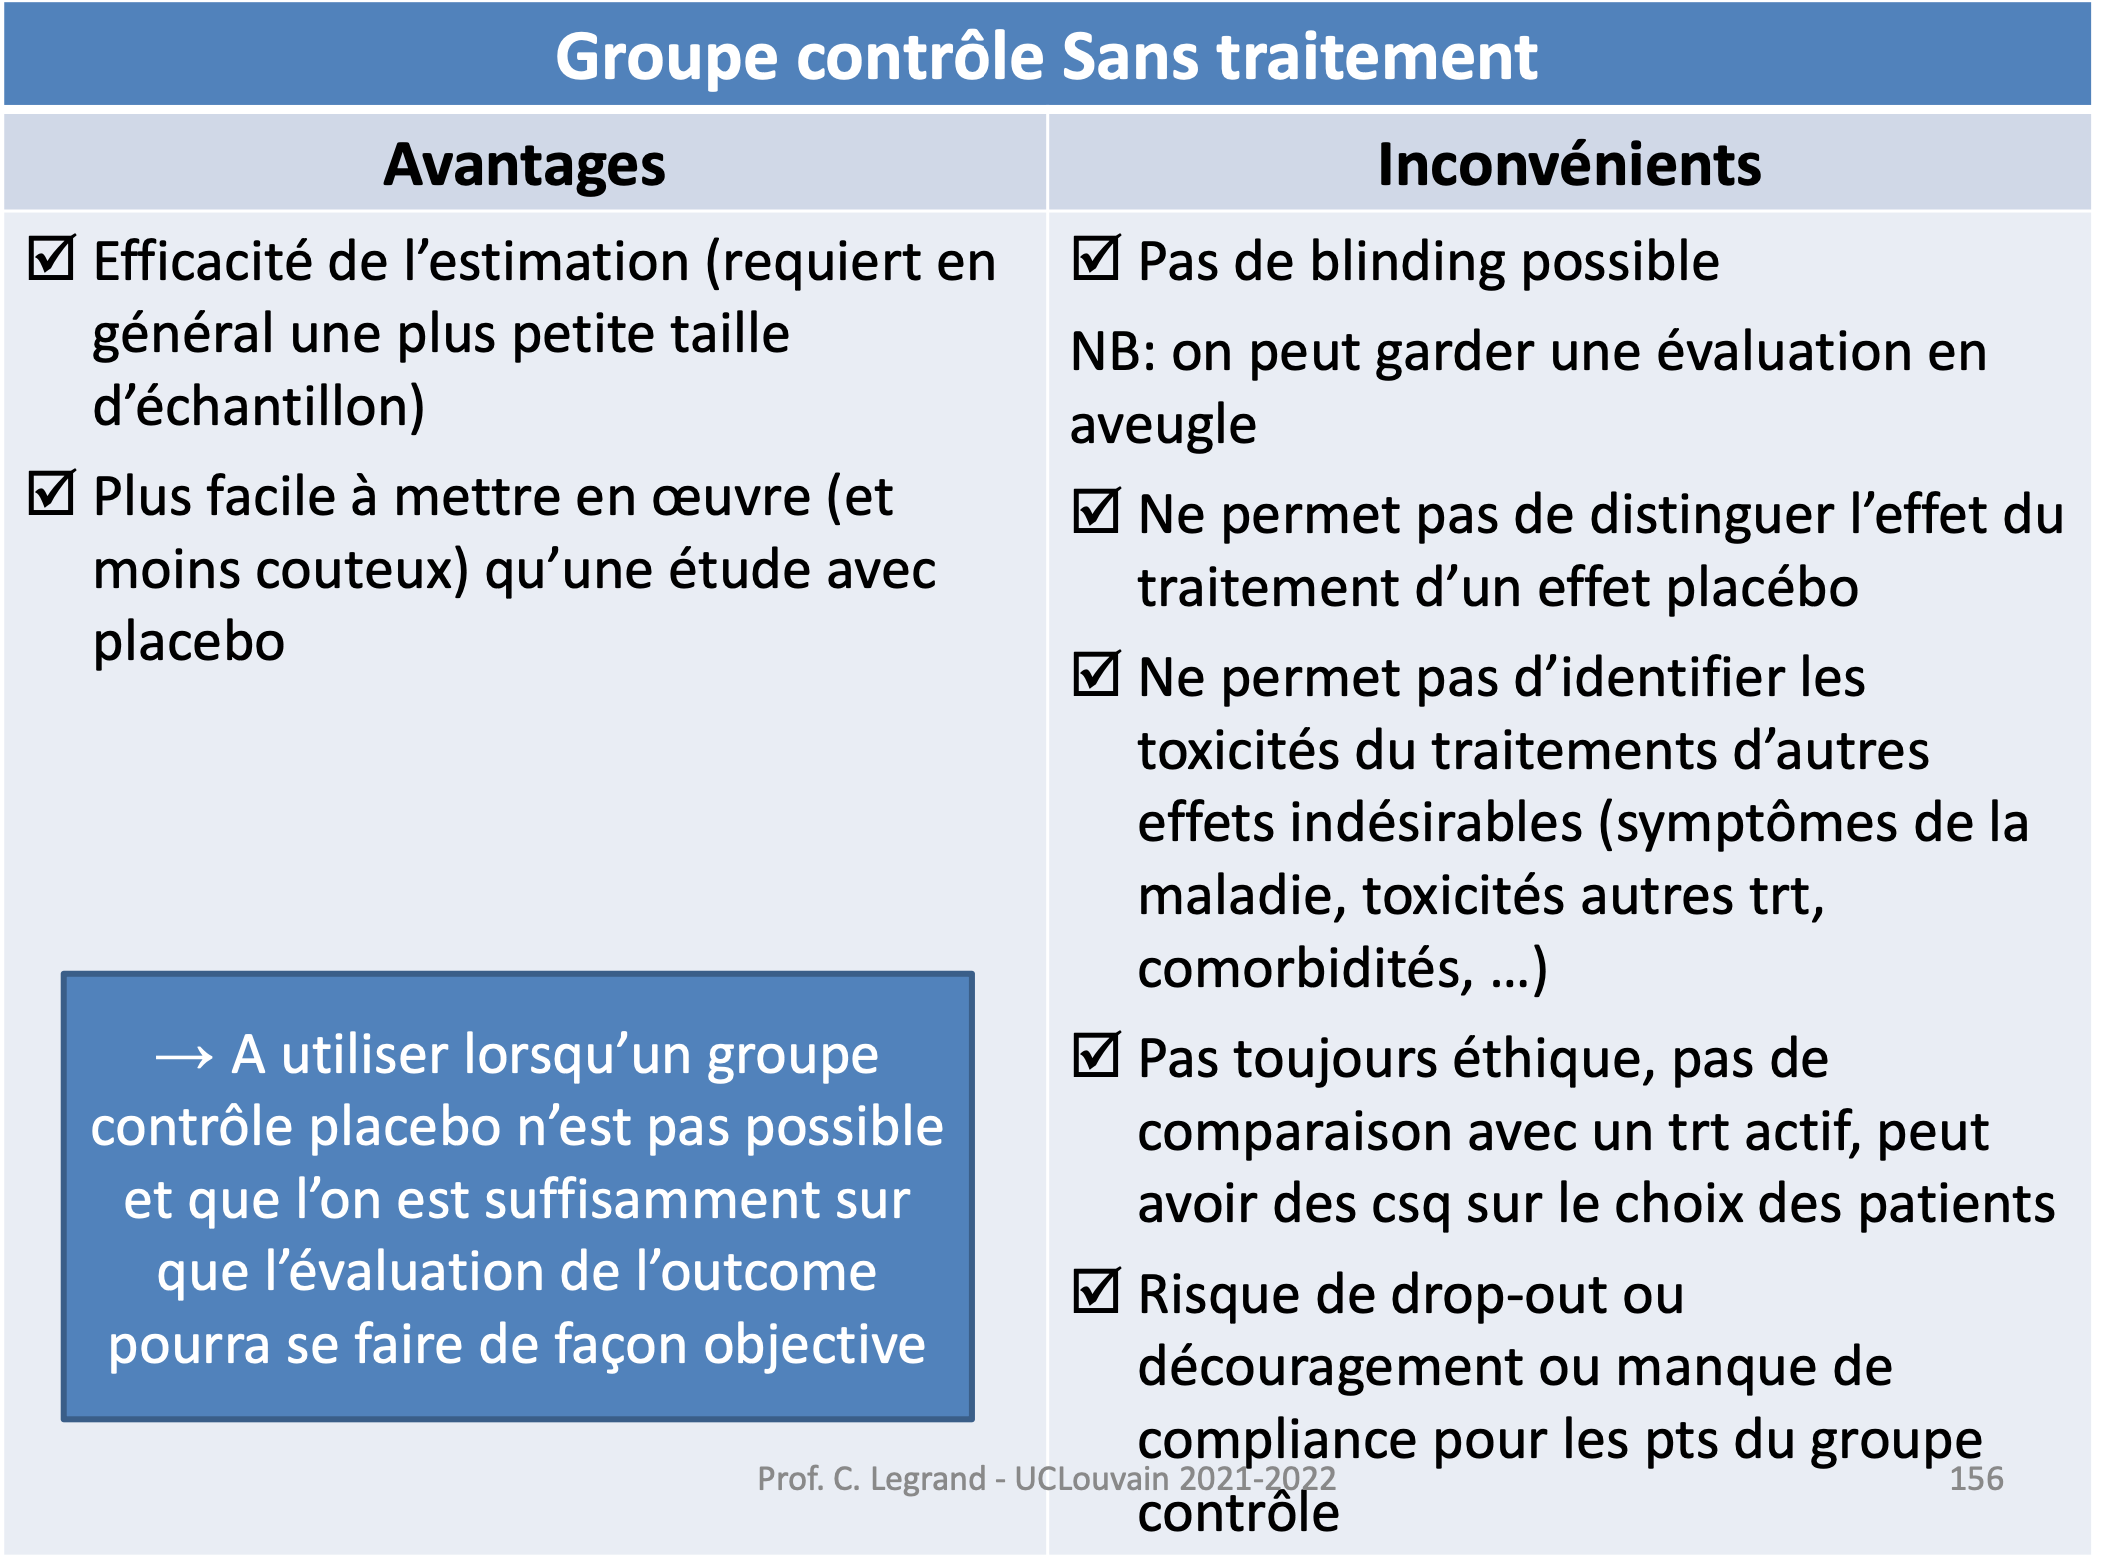
\includegraphics[scale=0.3]{images/no_treatment.png}
    \caption{}
    \label{fig:my_label}
\end{figure}

\section{Objectif de l’essai}

\subsection{Essai de Supériorité ou de Différence}
Le but est de déterminer si le traitement expérimental est plus efficace que le contrôle.

\begin{figure}[H]
    \centering
    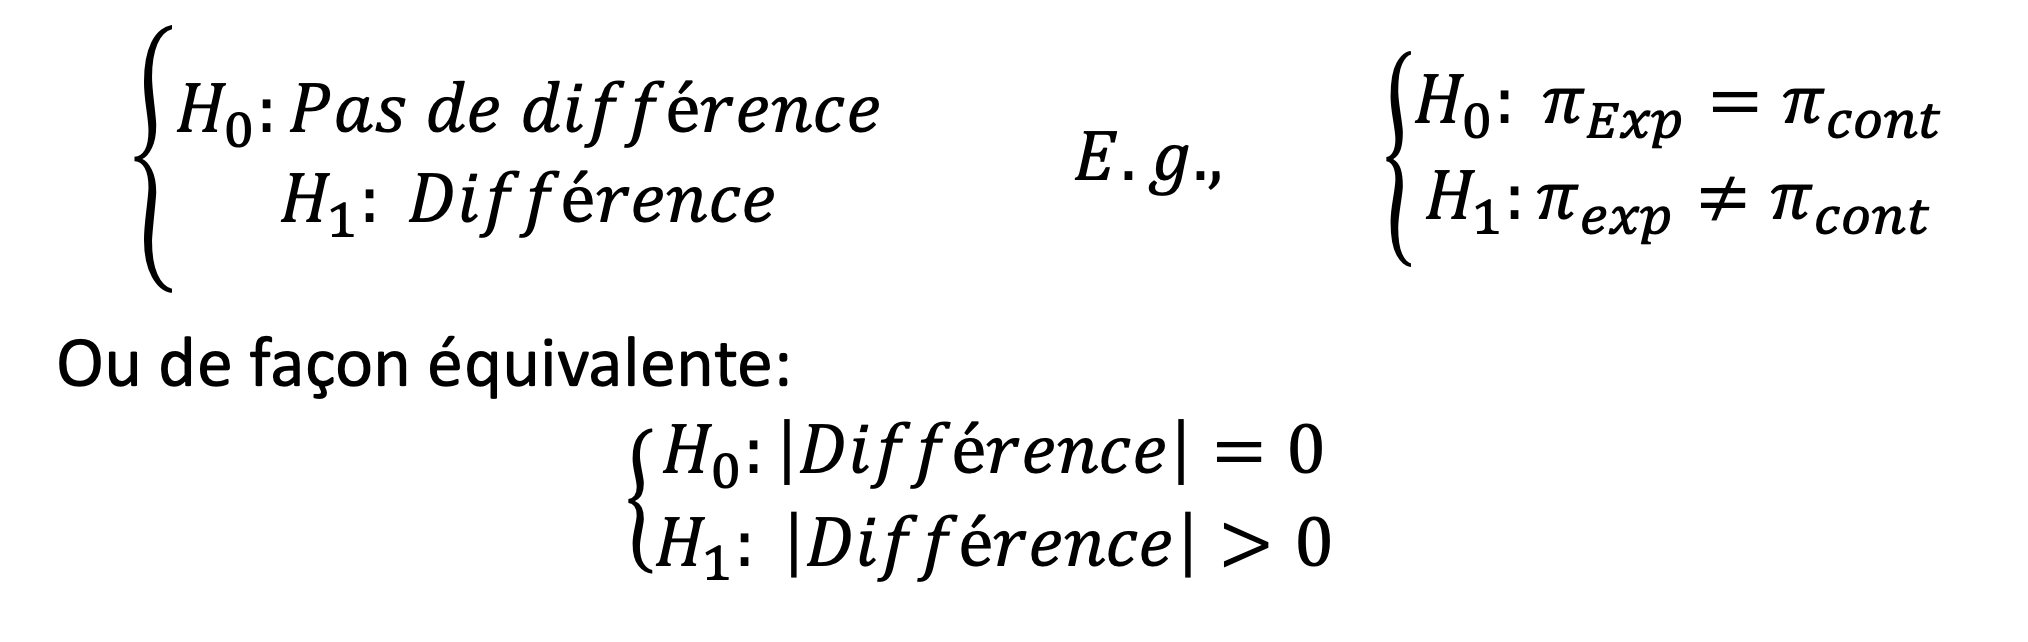
\includegraphics[scale=0.5]{images/essais_diff.png}
    \caption{}
    \label{fig:my_label}
\end{figure}

\textbf{Recommandations}\\

\begin{itemize}
    \item Choisir de faire un test bilatéral ou unilatéral en fonction de l’objectif de l’étude. On recommande en général de faire un test unilatéral uniquement lorsque la différence est d’office dans un sens.
    \item Choisir si le test sera bilatéral ou unilatéral avant d’avoir accès aux données de l’étude.
    \item Lorsque l’on présente une P-valeur, toujours spécifier à quel type de test celle-ci se rapporte.
    \item Toujours vérifier si un test est bilatéral ou unilatéral avant d’interpréter sa p-valeur et interpréter les résultats du test en fonction du type de test.
    \item Ne pas « surinterpréter » une p-valeur non significative
\end{itemize}

\subsection{Essai de Non-infériorité}
Déterminer si le traitement expérimental est "au moins aussi efficace" que le traitement standard, mais une des caractéristiques suivantes :
\begin{itemize}
    \item Moins agressif
    \item Moins toxique
    \item Moins invasif
    \item Moins couteux, plus faisable
\end{itemize}
Ces derniers points doivent être prouvés par \textbf{Endpoints secondaires}!

\begin{figure}[H]
    \centering
    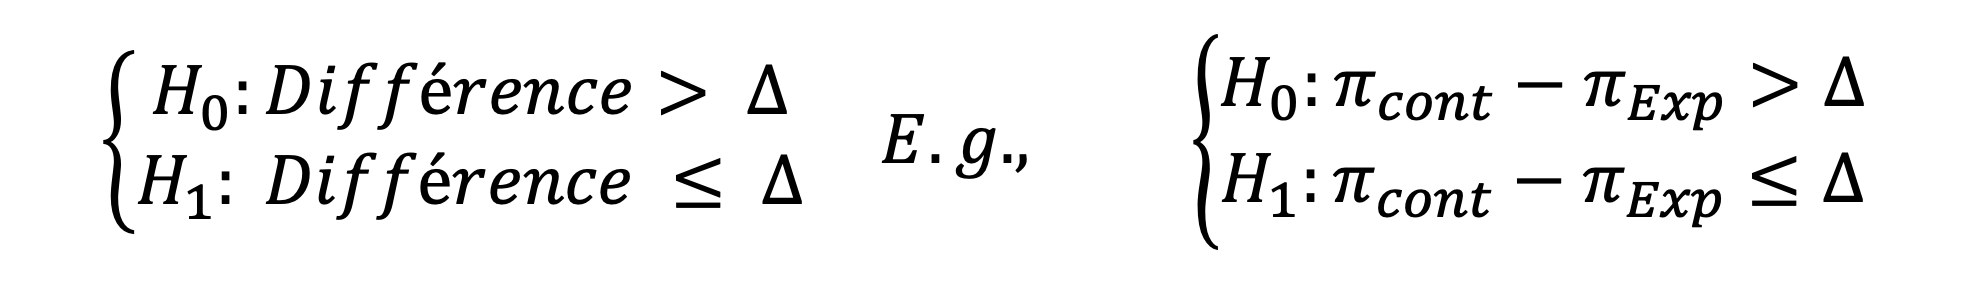
\includegraphics[scale=0.5]{images/nodiff.png}
    \caption{Hypothèse pour essai de non-infériorité}
    \label{fig:my_label}
\end{figure}

\textbf{Remarques}\\
\begin{itemize}
    \item Il s’agit donc clairement d’un test unilatéral, on verra que ce test est
souvent réalisé via le calcul d’un intervalle de confiance.
\item Si on démontre la non-infériorité, il faut obligatoirement montrer
l’avantage sur un autre endpoint.
\item Démontrer la non-infériorité contre un placebo ou un bras contrôle
non-actif n’a (en général) pas de sens
\end{itemize}


\subsection{Essai d’équivalence}
Déterminer si le traitement expérimental a la même efficacité que le traitement standard (ni moins bon, ni meilleur). Ces tests sont assez rares en recherche clinique et sont surtout utilisé pour les traitements « génériques ».

\begin{figure}[H]
    \centering
    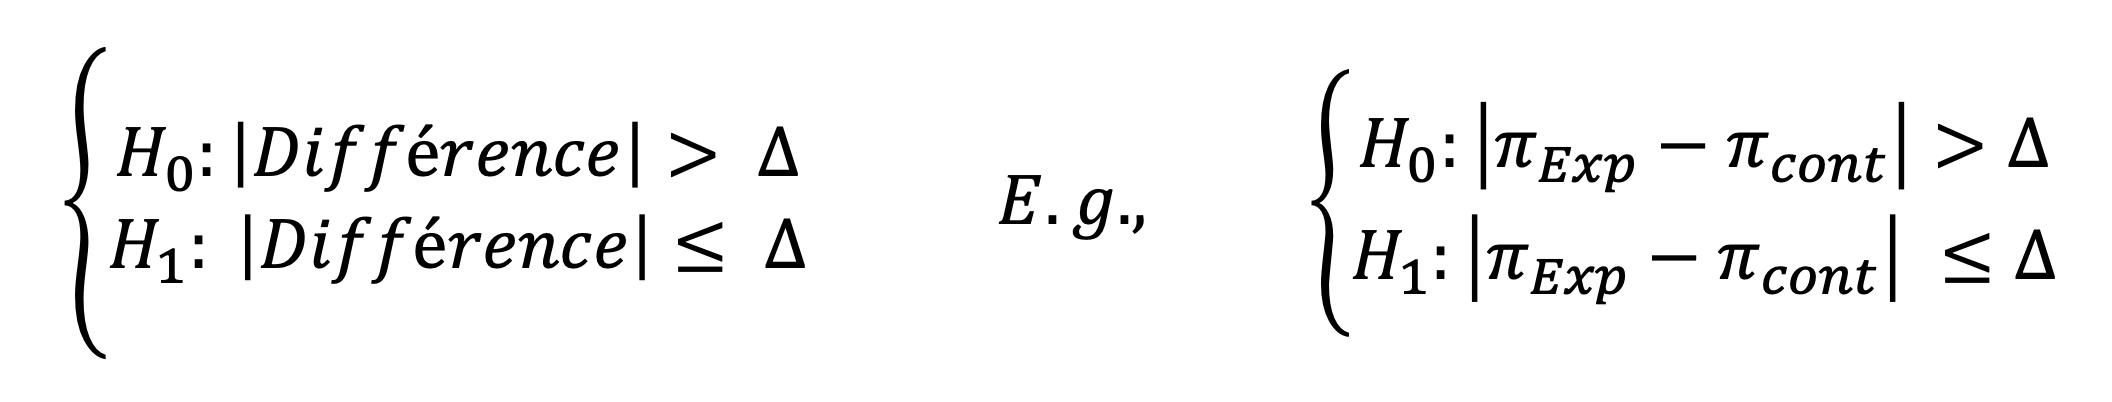
\includegraphics[scale=0.4]{images/equil.png}
    \caption{Hypothèse essai d'équivalence}
    \label{fig:essaisequi}
\end{figure}

\vspace{0.15cm}
\textbf{\textit{Peut-on conclure à la non-infériorité (ou
l’équivalence) au départ d’un essai clinique
de supériorité non significatif ?}}\\
On ne peut en général pas conclure la non-infériorité /
équivalence d’un essai clinique de supériorité non significatif. OK dans le cas particulier où une marge de non-infériorité $\Delta$ a
été prédéfinie dans le protocole.

\section{Plan d’expérience}

Le design d’un essai clinique de Phase III doit être choisi de façon à ce que l’essai ait un impact maximal sur la pratique clinique. Il doit avoir les caractéristiques suivantes :\\

\begin{itemize}
    \item simple, à grande échelle, multi-centrique (différents hôpitaux)
    \item randomisé (sauf maladie rare)
    \item endpoints approprié ("hard endpoint")
    \item suffisamment de puissance pour détecter une différence petite a modéré, mais cliniquement importante dans l’effet traitement
\end{itemize}


\begin{center}
    \textbf{ On donnera en général la préférence aux essais les plus simples}
\end{center}
Le plus simple il est, plus il sera facile de convaincre les autres des résultats du test.

On a différents designs de plan possibles.

Le premier est le \textbf{design parallèle à 2 groupes}. 
\begin{figure}[H]
    \centering
    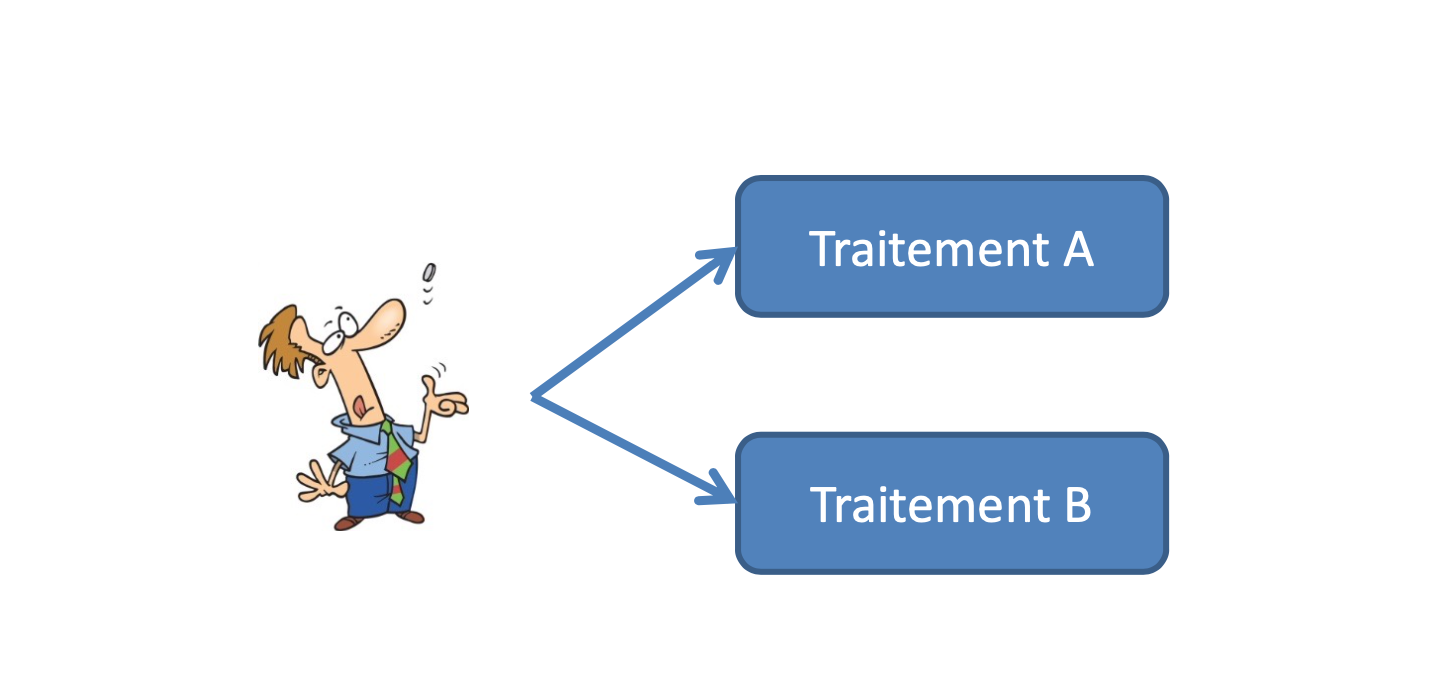
\includegraphics[scale =0.2]{images/2treatments.png}
    \caption{design parallèle à 2 groupes}
    \label{fig:design2}
\end{figure}

Le second est le \textbf{design parallèle à plus de 2 groupes}. Dans le cas de ce design, il est plus difficile de définir les hypothèses pour les tests. 
\begin{figure}[H]
    \centering
    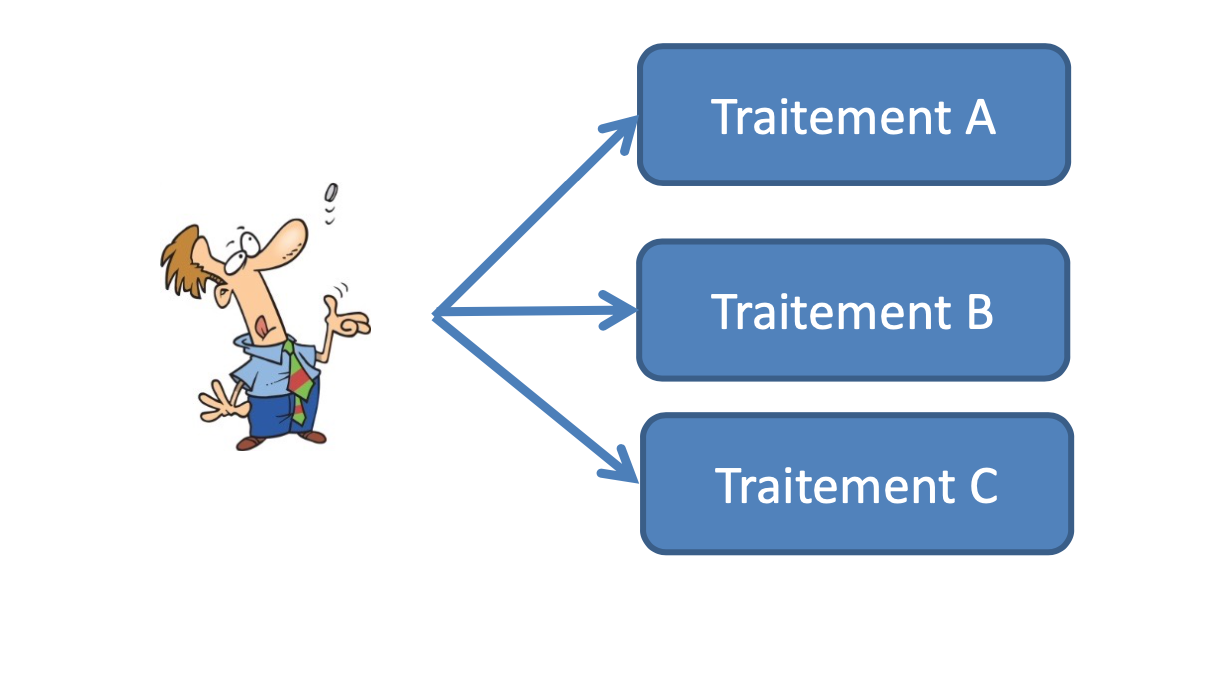
\includegraphics[scale =0.2]{images/more2.png}
    \caption{design parallèle à plus de 2 groupes}
    \label{fig:my_label}
\end{figure}

Il existe des designs plus compliqués où on a en parallèle plusieurs groupes et on réalise en plusieurs étapes les essais.Exemple : MAM (multiple arm) trial.

On a aussi le \textbf{design factoriel 2x2}. Ici, on doit avoir comme hypothèse qu'il n'y a pas d'interaction entre les traitements testés dans les 2 essais.
\begin{figure}[H]
    \centering
    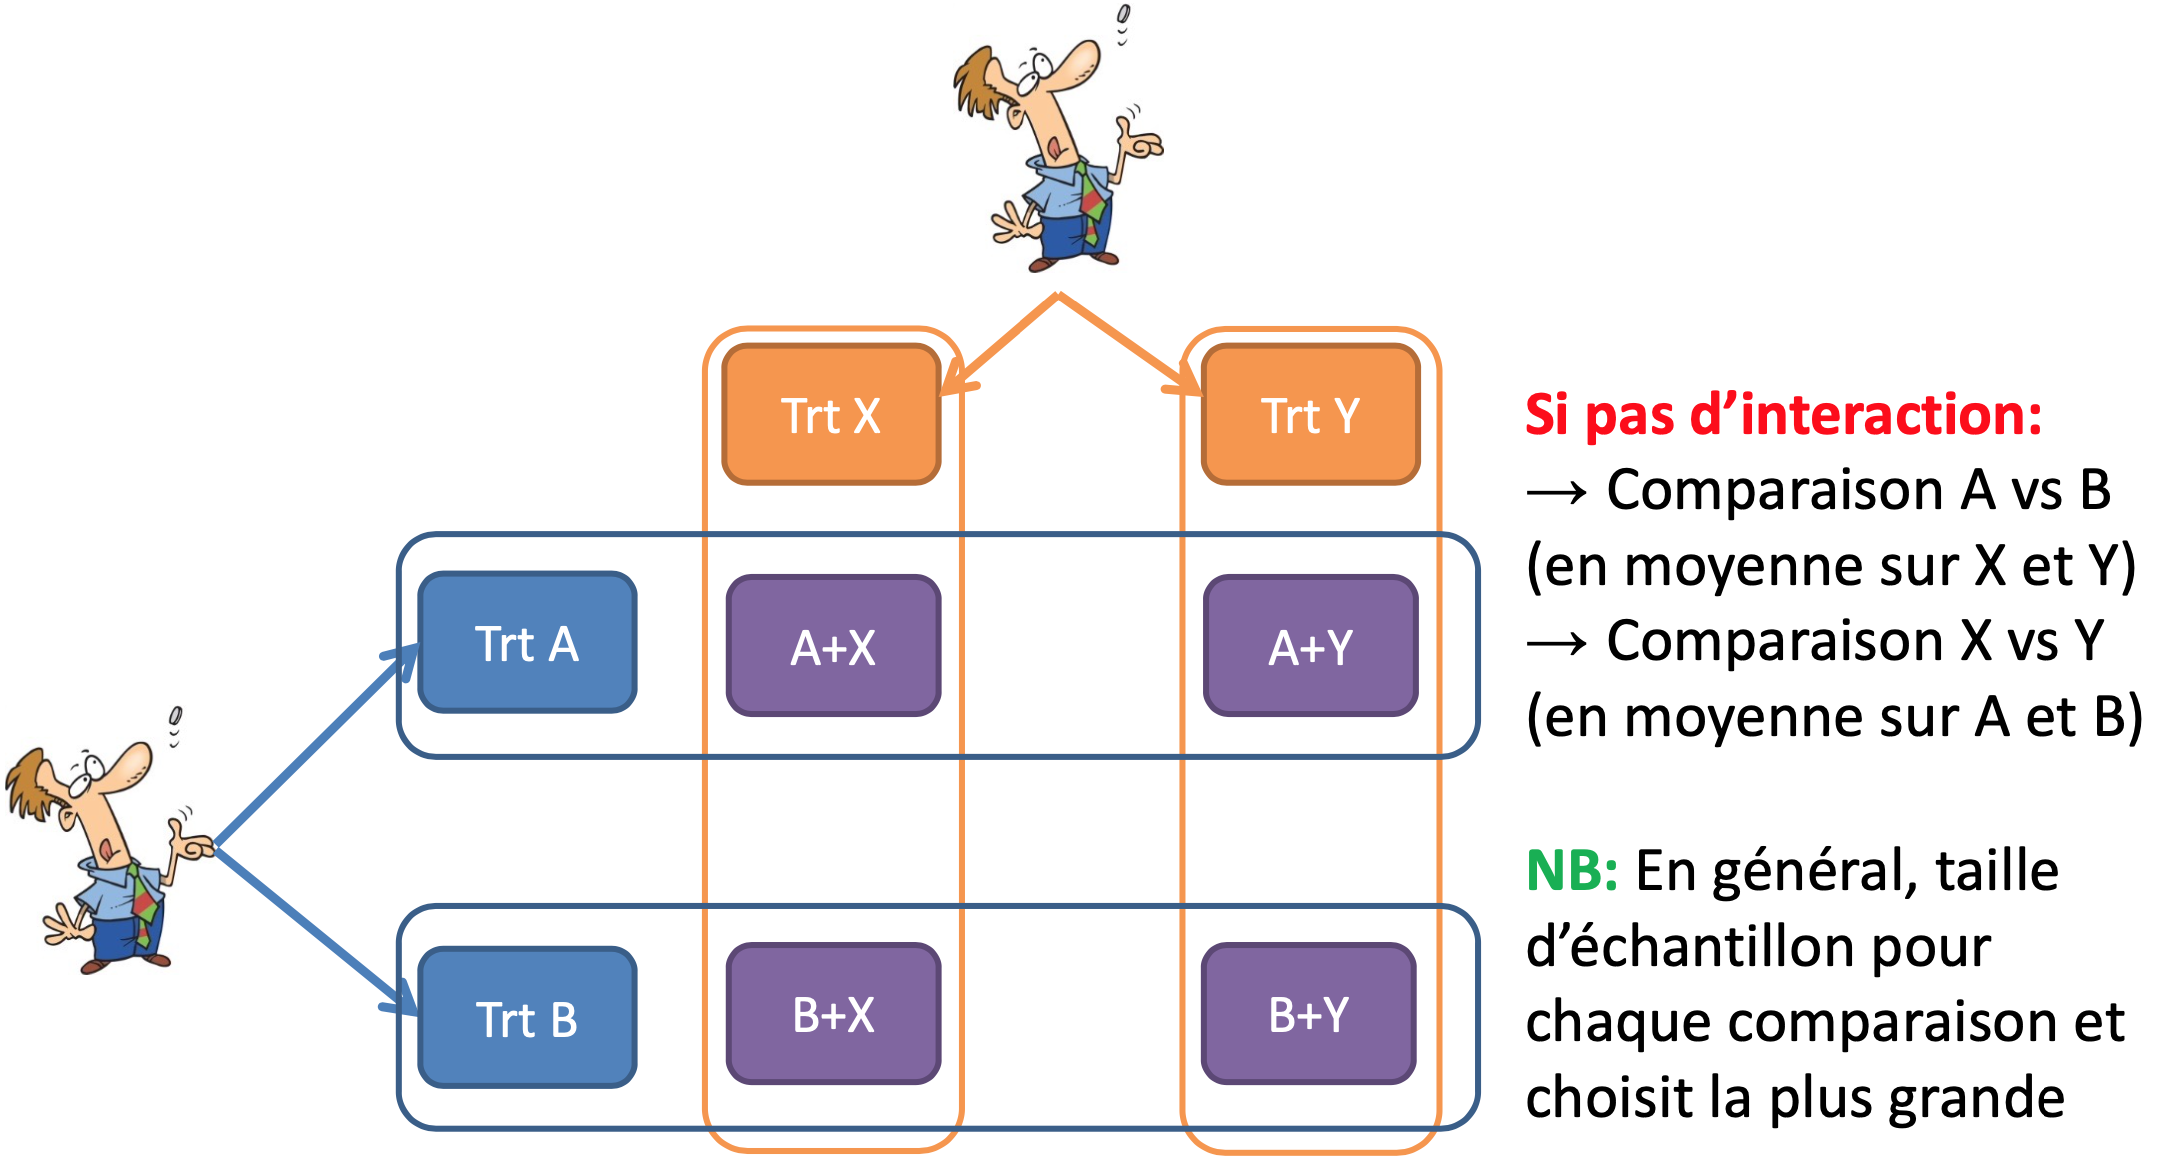
\includegraphics[scale = 0.2]{images/parallel.png}
    \caption{design factoriel 2x2}
    \label{fig:designfactoriel}
\end{figure}

Enfin, on a le \textbf{design cross-over}. Le patient va recevoir tous les traitements, mais dans des ordres différents. Cela a comme effet de diminuer la variabilité, car on fait des comparaisons \textbf{intra-patient}. Le patient est son propre contrôle. Le grand avantage est qu'on a besoin d'un échantillon réduit, mais les techniques de statistiques doivent être adaptées. 
Quelques hypothèses pour ce type de design :
\begin{itemize}
    \item Ordre dans lequel on donne les traitements n'a pas d'importance.
    \item Patients dans le même état avant de commencer chaque période. On n'a pas une dégradation ou une guérison entre les différentes phases.
    \item On travaille sur des endpoints à court terme. 
\end{itemize}


\begin{figure}[H]
    \centering
    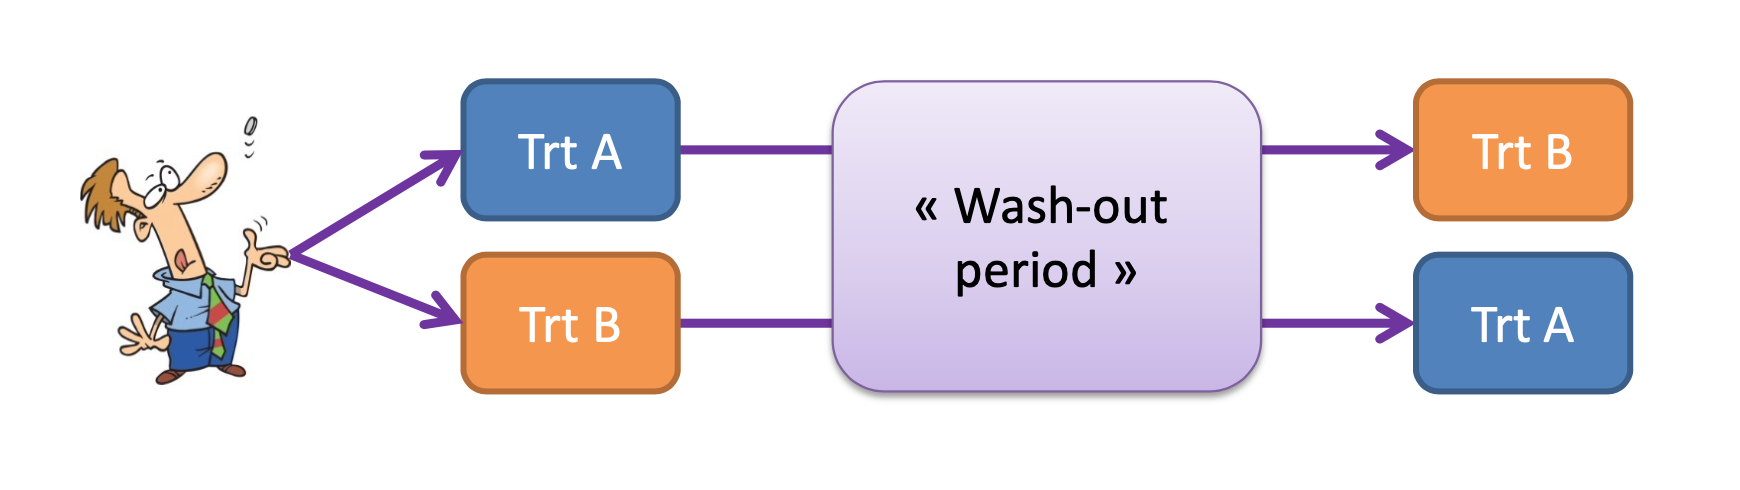
\includegraphics[scale =0.2]{images/overcrossing.png}
    \caption{design cross-over}
    \label{fig:my_label}
\end{figure}



\section{Sélection des patients}
Dernière phase du développement clinique d’un nouveau traitement. \textbf{La définition de la population d’intérêt est cruciale}. On va faire un compromis entre aussi que possible et très restrictif.

\begin{figure}
    \centering
    \includegraphics{}
    \caption{sélections des patients : compromis entre les deux situations}
    \label{fig:my_label}
\end{figure}


\section{Monitoring et IDMC}
La randomisation des patients entre les différents traitements n’est éthiquement acceptable que si le médecin (et de façon générale la communauté scientifique) est en état d’équipoise \footnote{L’équipoise du médecin-chercheur, cet état de réelle incertitude quant aux mérites respectifs de deux traitements à comparer, est, du moins théoriquement — parce qu’impossible dans l’absolu —, l’une des exigences éthiques de l’essai clinique, tout comme l’est l’adoption d’une méthodologie qui respecte les canons de la science.}.\\
Pendant le cours d'un essai clinique, il peut devenir claire que :
\begin{itemize}
    \item soit pour certains/tous les patients un des traitements est meilleur que les autres.
    \item soit que le traitement est trop toxique pour certains/tous les patients.
\end{itemize}

Dans ce cas, on n'est pas dans un état d'équipoise et donc il est nécessaire de stopper l'essai clinique même si cela entraine des conséquences négatives.

C'est pour cela qu'on fait appel à des gens extérieurs pour cette étape.





